\documentclass[border=6pt]{standalone}
\usepackage{amsmath}
\usepackage{amssymb}
\usepackage{tikz}
\usepackage{pgfplots}
\pgfplotsset{compat=1.18}
\usetikzlibrary{arrows.meta,calc,positioning}
\begin{document}
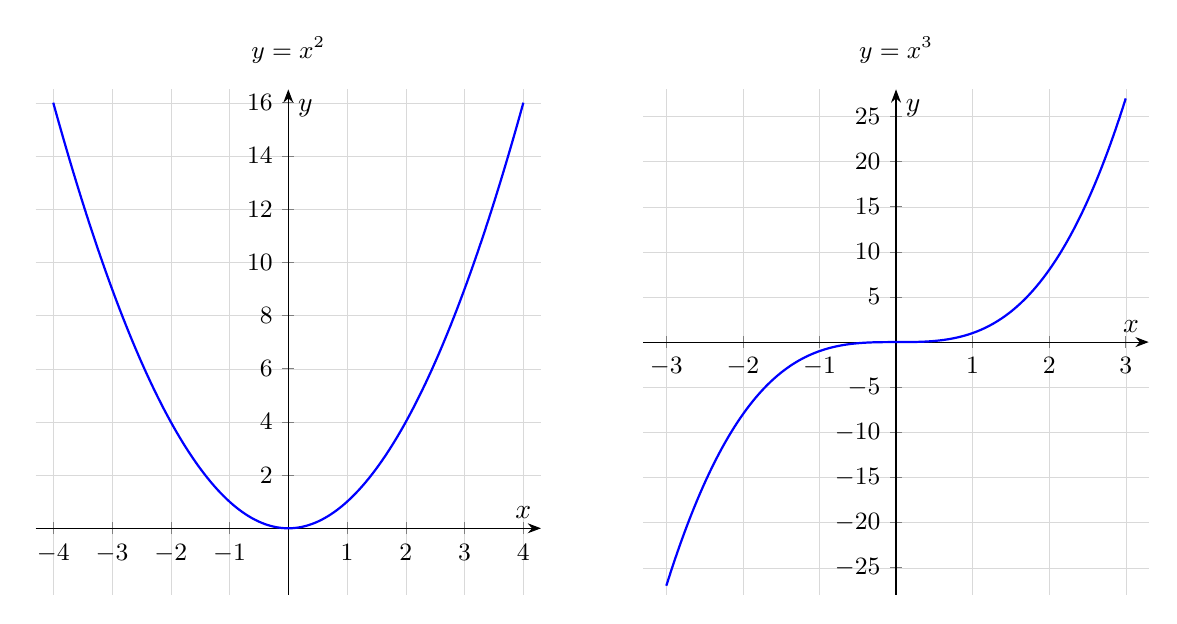
\begin{tikzpicture}
\begin{axis}[name=ax1,
    axis lines = middle,
    xlabel = {$x$}, ylabel = {$y$},
    grid=both,
    grid style={line width=.1pt, draw=gray!30},
    axis line style={-Stealth},
    legend style={font=\small},
    tick label style={font=\small},
    xmin=-4.3, xmax=4.3, ymin=-2.5, ymax=16.5,
    xtick={-4,-3,-2,-1,0,1,2,3,4},
    ytick={0,2,4,6,8,10,12,14,16},
    width=8cm, height=8cm,
    title={\small $y=x^2$},
]
\addplot[domain=-4:4, samples=150, thick, blue] {x^2};
\end{axis}
\begin{axis}[at={(ax1.south east)}, anchor=south west, xshift=1.3cm,
    axis lines = middle,
    xlabel = {$x$}, ylabel = {$y$},
    grid=both,
    grid style={line width=.1pt, draw=gray!30},
    axis line style={-Stealth},
    legend style={font=\small},
    tick label style={font=\small},
    xmin=-3.3, xmax=3.3, ymin=-28, ymax=28,
    xtick={-3,-2,-1,0,1,2,3},
    ytick={-25,-20,-15,-10,-5,0,5,10,15,20,25},
    width=8cm, height=8cm,
    title={\small $y=x^3$},
]
\addplot[domain=-3:3, samples=150, thick, blue] {x^3};
\end{axis}
\end{tikzpicture}
\end{document}
